\documentclass[11pt,a4paper]{article}

% Define page geometry
\usepackage{geometry}
\geometry{left=2.2cm,
	right=2.2cm,
	top=2.2cm,
	bottom=2cm}
\parskip 0.15cm
\setlength{\parindent}{0cm}
\usepackage{pdflscape}
\usepackage[document]{ragged2e}

% Set font
\usepackage[T1]{fontenc}

% Image handling
\usepackage{graphics}  % Insert images easily
\usepackage{graphicx}  % Extended image support

\makeatletter
	\g@addto@macro\@floatboxreset\centering  % Automatically centre images (floats)
\makeatother

\graphicspath{ {img/} }
\usepackage{float}  %  Graphics placement [H] [H!] arguments
\usepackage{subfig}  % Compound figures

% Tables
\usepackage{multirow}
\usepackage{longtable}

% Bibliography management
\usepackage{natbib}    % Bibliography management - Use author/date citations
\bibliographystyle{agsmnourl}  % Use custom agsm bibliography template with no URL
\usepackage{cite}  % Citation options

% Text formatting
\usepackage{url} % Allow nice formatting of URLs in text

\usepackage{enumerate}  % Enumerated lists

\usepackage{lineno}  % Line numbers

\usepackage{textcomp}
\newcommand{\textapprox}{\raisebox{0.5ex}{\texttildelow}}  % Command for a good tilde

\usepackage{siunitx}
\usepackage{amsmath}

\usepackage{xcolor}
\newcommand{\todo}[1]{\textcolor{red}{\textbf{#1}}}   % \todo{NOTE TO SELF WRITTEN IN RED}

% Custom title formatting
\let\oldtitle\title

\renewcommand{\title}[1]{\oldtitle{\vspace{-1.5cm}#1}}

\usepackage[breaklinks]{hyperref}
\definecolor{links}{RGB}{191,59,72}
\hypersetup{
	breaklinks,
	colorlinks,
	allcolors=links,
	linktoc=section,
	pdfauthor={John L. Godlee}
}
\def\subsectionautorefname{section}
\def\subsubsectionautorefname{section}
% \usepackage{biblatex}

\usepackage{lineno}
\linenumbers

\newcommand{\titletext}{Phenology and diversity in Zambia}

\newcommand{\censusDate}{2014}
\newcommand{\nTotalSites}{993}
\newcommand{\modisSLC}{0.05}
\newcommand{\trmmSLC}{0.06}
\newcommand{\plotDistPer}{93.9}
\newcommand{\nscaInertia}{1.81}
\newcommand{\mopanePer}{50}
\newcommand{\stemsHa}{50}
\newcommand{\stemSize}{10}
\newcommand{\nSites}{709}


\begin{document}

{\LARGE{Title: \titletext}}

\vspace{1cm}

Authors: Godlee, J. L.\textsuperscript{1}, 

\textsuperscript{1}: School of GeoSciences, University of Edinburgh, Edinburgh, United Kingdom \\
\textsuperscript{2}: Some other address

\vspace{1em}
Corresponding author:

John L. Godlee

johngodlee@gmail.com

School of GeoSciences, University of Edinburgh, Edinburgh, United Kingdom

\section{Acknowledgements}

\newpage{}

%{\LARGE{\textbf{Blinded Main Text File}}}

\LARGE{Title: \titletext}

\normalsize{Running title: \titletext}

\section{Abstract}

\section{Introduction}

The seasonal timing of tree leaf production in deciduous woodlands directly influences ecosystem-level productivity \citep{}. Leaf Area Index (LAI) is tightly coupled with photosynthetic activity and therefore gross primary productivity in these ecosystems \citep{}. Previous studies have shown that diurnal temperature variation and precipitation are the primary determinants of tree phenological activity in water-limited savannas \citep{}. At regional spatial scales, woodland phenological activity can be predicted well using only environmental factors \citep{}, but local variation exists in leaf production cycles which cannot be attributed solely to environment \citep{}. Previously, it has been shown that leaf phenological responses to the onset of rainfall vary among deciduous woodlands of different vegetation type \citep{}.

Tree species vary in their life history strategy with regards to the timing of leaf production \citep{}. In tropical deciduous woodlands, tree species vary in their leaf production in response to the onset of seasonal rainfall and the end of the rainy season \citep{}. More conservative species (i.e. slower growing, robust leaves, denser wood) tend to green-up before rainfall has commenced, and can often persist after the rainy season has finished despite having lower overall productivity, while less conservative species tend to green-up during the rainy season, and create a dense leaf-flush during the mid-season peak of growth. It has been suggested that this variation in leaf phenological activity between species is one aspect by which increased tree species richness causes an increase in ecosystem-level productivity in deciduous woodlands \citep{}. Building on research linking biodiversity and ecosystem function, one might expect that an ecosystem with a wider diversity of tree species might be better able to maintain consistent leaf coverage for a longer period over the year, as species vary in their optimal growing conditions due to niche complementarity, whereby coexisting species vary in their occupation of niche space due to competitive exclusion \citep{}. In addition, in water-limited woodland-savannas such as those found in large areas of southern Africa, the ability to maintain more consistent leaf coverage over the growing season may provide facilitative effects to other tree species that are less well-adapted to moisture-limiting conditions, but are more productive, by providing shade and influencing below ground water availability through hydraulic lift \citep{}.

In the deciduous woodlands of Zambia, a highly pronounced single wet-dry season annual oscillation is observed across the majority of land area, with local exceptions in some mountainous areas \citep{}. Variation in leaf phenological activity across the region therefore has a large influence on annual gross primary productivity, with important consequences for the global carbon cycle, in addition to having local consequences for human inhabitance that benefit from the harvest of woodland products \citep{}. Savanna woodlands of a number of different types (species composition and structure) are found across the region, but these are often poorly differentiated in regional-scale studies \citep{}, resulting in a dearth of information on the phenological behaviour of different woodlands.

In this study we contend that, across Zambian deciduous woodlands, tree species composition and tree species diversity influence four key measurable aspects of the tree phenological cycle: (1) the rate of greening at the start of the seasonal growth phase, (2) the overall length of the growth period, and (3) the rate of senescence at the end of the seasonal growth phase, together affecting cumulative gross primary productivity over the course of the growing season. It is hypothesised that: (H\textsubscript{1}) due to variation among species in minimum viable water availability for growth, plots with greater species richness will exhibit a slower rate of greening, with the start of the growing season occuring earlier with respect to the onset of rain. Additionally, we hypothesise that: (H\textsubscript{2}) plots with greater species richness will exhibit a longer growth period and greater cumulative green-ness over the course of the growth period, due to a higher resilience to variation in water availability, acting as a buffer to ecosystem-level productivity. Finally, we hypothesise that: (H\textsubscript{3}) irrespective of species diversity, variation in tree species composition and vegetation type will cause variation in growth season length. 

\section{Materials and methods}

\subsection{Data collection}

We used plot-level data on tree species diversity across \nSites{} sites from the Zambian Integrated Land Use Assessment Phase II (ILUA-II), conducted in \censusDate{} \citep{}. Each site consisted of four 20x50 m (0.2 ha) plots positioned radially around a central point, with a distance of 300 m from the central point to the centre of each plot \autoref{schematic}. The original census contained \nTotalSites{}, which was filtered in order to define study bounds and to ensure data quality. Only sites with >\stemsHa{} stems ha\textsuperscript{-1} were included in the analysis, to ensure all sites represented woodland rather than “grassy savanna”, which is considered a separate biome with very different species composition and ecosystem processes governing phenology \citep{Parr2014}. Sites in Mopane woodland were removed by filtering sites with greater than \mopanePer{}\% of trees belonging to \textit{Colophospermum mopane}, preserving only plots with Zambesian tree savanna / woodland. Mopane woodlands \todo{have different processes governing their phenology, so it's not sensible to include them}. 
\begin{figure}[H]
\centering
	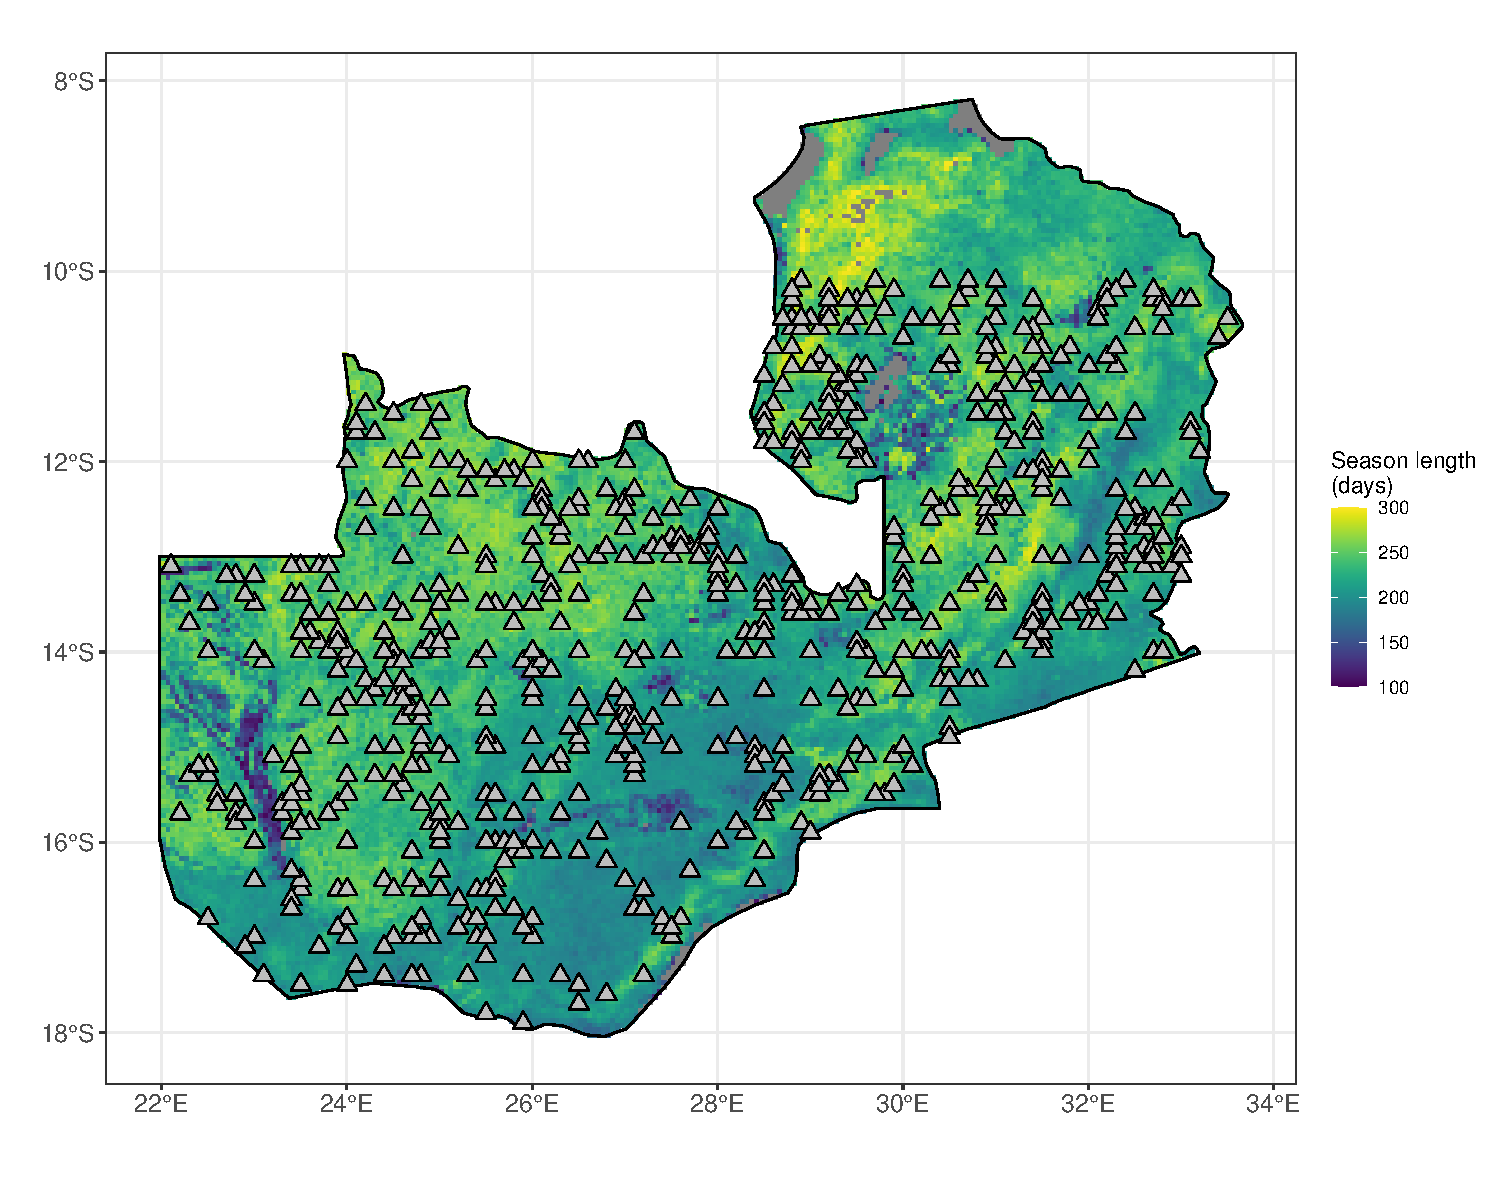
\includegraphics[width=0.8\textwidth]{plot_loc}
	\caption{Distribution of study sites within Zambia as white triangles, each consisting of four plots. Zambia is shaded according to growing season length as estimated by the MODIS VIPPHEN product, at 0.05 degrees spatial resolution.}
	\label{plot_loc}
\end{figure}

\begin{figure}[H]
\centering
	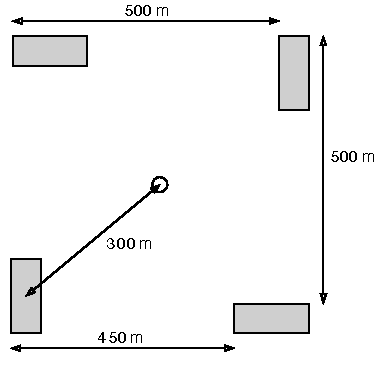
\includegraphics[width=0.5\textwidth]{schematic.drawio}
	\caption{Schematic diagram of plot layout within a site. Each 20x50 m (0.2 ha) plot is shaded grey. The site centre is denoted by a circle. Note that the plot dimensions are not to scale.}
	\label{schematic}
\end{figure}

Within each plot, the species of all trees with at least one stem >5 cm diameter at breast height (DBH) were recorded. Plot data was aggregated to the site level for analyses to avoid pseudo-replication caused by the more spatially coarse phenology data. Tree species composition varied little among the four plots within a site, and were treated as representative of the woodland in the local area.

Climatic variables were derived from the WorldClim database, using the BioClim variables, with a pixel size of 30 arc seconds (926 m at the equator) \citep{Fick2017}. Mean Annual Precipitation (MAP) was calculated as the yearly sum of daily precipitation, averaged across all years of available data (1970-2000). Mean diurnal temperature range (Diurnal $\delta$T) was calculated as the mean of monthly temperature range. 

To quantify phenology at each site, we used the MODIS MOD13Q1 satellite data product at 250 m resolution \citep{}. The MOD13Q1 product provides an Enhanced Vegetation Index (EVI) time series at 16 day intervals. EVI is well-correlated with gross primary productivity and so can act as a suitable proxy \citep{}. We used all scenes from January 2015 to August 2020 with less than 20\% cloud cover.

All sites were determined to have a single annual growth season according to the MODIS VIPPHEN product \citep{}, which assigns pixels of 0.05 decimal degrees up to three growth seasons per year. For each site, we split the fitted EVI time series into growth season chunk, each centred on a peak of EVI values. We fit a single loess model with a span of \loessSpan{} across these growth season chunks to generate an average growth season curve. We estimated the start of the growing season as the day of the year at which EVI rises 10\% above the minimum EVI value in the curve, and the end of the growing season when EVI falls below 10\% of the minimum EVI value. We estimated the length of the growing season as the number of days between the start and end of the growing season. We estimated the greening rate as the slope of a linear model across EVI values between the start of the growing season and the maximum EVI value reached during the growing season. Similarly the senescence rate was estimated as the slope of a linear model between the maximum EVI and the end of the growing season \autoref{ts_example}.

\begin{figure}[H]
\centering
	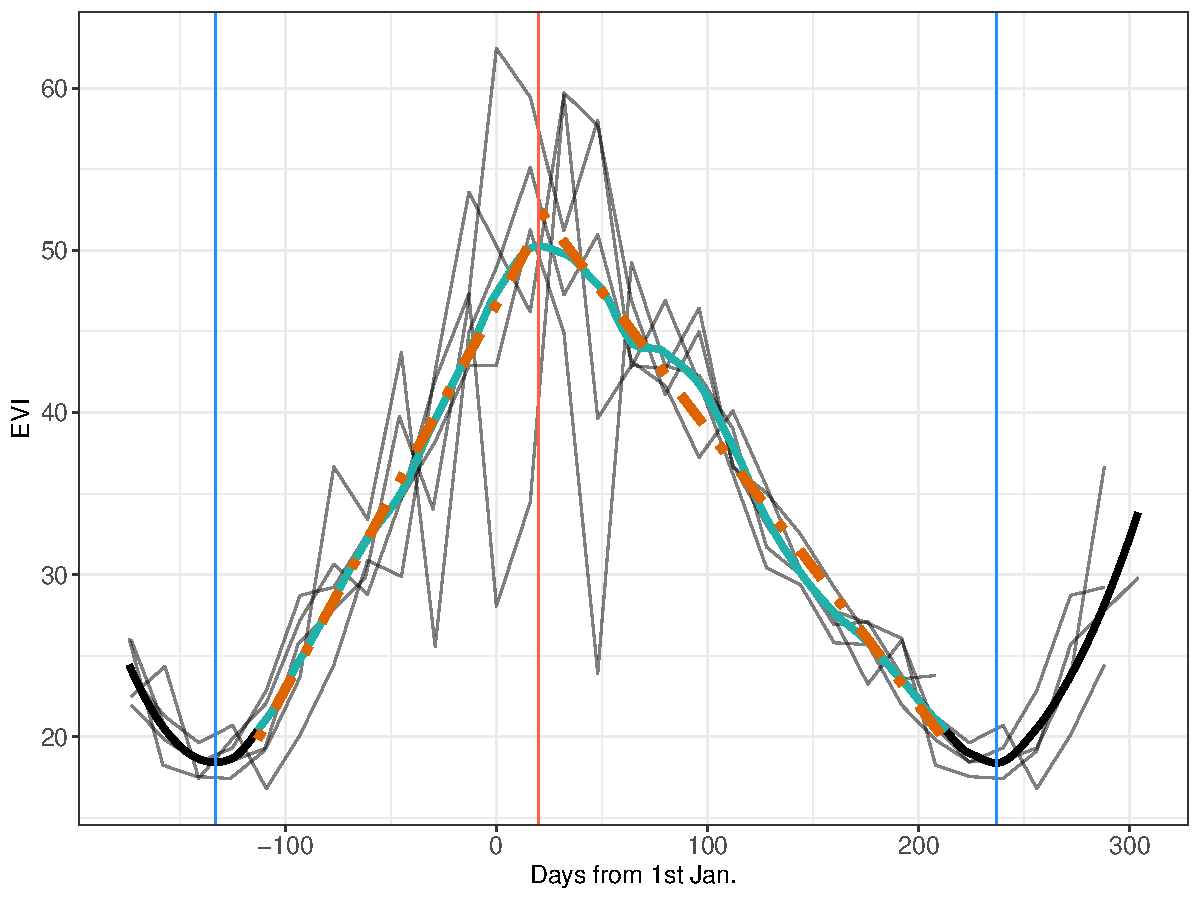
\includegraphics[width=0.8\textwidth]{ts_example}
	\caption{Example EVI time series, demonstrating the metrics derived from it. Thin black lines show the raw EVI time series, with one line for each annual growth season. The thick black line shows the loess model fit. The thin blue lines show the minima which bound the growing season. The red line shows the maximum EVI value reached within the growing season. The shaded cyan area of the loess fit shows the growing season, during which the EVI is above 10\% of the background level. The two orange dashed lines are linear regressions predicting the greening rate and senescence rate at the start and end of the growing season, respectively. Note that while the raw EVI time series fluctuate greatly around the middle of the growing season, mostly due to cloud, the loess fit effectively smooths this variation to estimate the true average EVI during the mid-season period.}
	\label{ts_example}
\end{figure}


\subsection{Data analysis}

To quantify variation in tree species composition we computed a Principle Coordinate Analysis (PCoA), with Cailliez correction for potential negative eigenvalues \citep{Legendre1998}, on a Bray-Curtis dissimilarity matrix calculated from tree species abundance per site, using the \texttt{ape} R package \citep{ape2019}. The first three axes of this PCoA explained \pcoaPer{} of the variation in species composition among sites according to eigenvalue analysis. These three axes were used in further statistical modelling.

We used multivariate linear models with a spatial autocorrelation term, using the \texttt{spaMM} R package \citep{spaMM2014}, to assess the role of tree species diversity on each of the three chosen phenological metrics. We defined a maximal model structure including tree species richness, tree species abundance evenness, the first 4 principle coordinate analysis axes of tree species composition, and climatic variables shown by previous studies to strongly influence phenology. The maximal model was compared to a null model containing only climatic variables using a likelihood ratio test and by comparison of marginal and conditional AIC values. All models were fitted using Maximum Likelihood to allow comparison of fixed effects \citep{}. Explanatory variables in each model were transformed to achieve normality where necessary and standardised to Z-scores prior to modelling. Spatial autocorrelation structures were fitted using a Mat\`{e}rn correlation model \citep{}.

Hierarchical partitioning was used to assess the independent and joint effects of each independent variable in the maximal model for each phenological metric \citep{Chevan1991, MacNally2002}, using the \texttt{hier.part} R package \citep{hier.part2004}. Hierarchical partitioning calculates goodness-of-fit across all combinations of independent variables \citep{Walsh2013} and is used to estimate their independent contribution to model fit \citep{MacNally2002}. This method was chosen because of its effectiveness in accounting for model multicollinearity \citep{Olea2010}. 

All statistical analyses were conducted in R version 4.0.2 \citep{R2020}.

\section{Results}

Species composition, richness and evenness had significant effects on cumulative EVI, greening rate and senescence rate \autoref{mod_spamm_slopes}. Hierarchical partitioning demonstrated that MAP and Diurnal $\delta$T had strong independent contributions to all phenological metrics except senescence rate. 

The models with species diversity terms for cumulative EVI, greening rate and senescence rate were all of better quality than equivalent models including only MAP and Diurnal $\delta$T, while the model for season start date was not significantly better, and the model for season length was of worse quality \autoref{spamm_stat}. 

Species richness had a negative effect on season start day and greening rate, as expected. Sites with higher species richness tended to have an earlier season start day and a shallower greening rate slope. 

While MAP had stong significant effects on all other phenological metrics, it did not have a significant effect on cumulative EVI.

Contrary to our predictions, richness and evenness had a negative effect on cumulative EVI.

Species composition tended to have a stronger effect on all phenological metrics than species richness. Senescence rate imparticular was heavily affected by PCoA 3, which described variation in \todo{how to describe contents of a PCOA axis?}.

% latex table generated in R 4.0.2 by xtable 1.8-4 package
% Fri Sep  4 14:54:10 2020
\begin{table}[ht]
\centering
\begin{tabular}{rccccc}
  \hline
Predictor & Cumulative EVI & Season length & Greening rate & Senescence rate & Season start \\ 
  \hline
Richness & 1.33 & 10.62 & 6.29 & 3.18 & 9.42 \\ 
  Evenness & 0.11 & 0.38 & 0.86 & 3.20 & 0.38 \\ 
  Stem density & 2.37 & 0.66 & 0.64 & 1.35 & 2.13 \\ 
  PCoA 1 & 6.59 & 15.14 & 31.50 & 6.37 & 9.78 \\ 
  PCoA 2 & 4.33 & 4.98 & 2.16 & 0.68 & 3.17 \\ 
  PCoA 3 & 45.30 & 3.46 & 34.13 & 82.16 & 6.17 \\ 
  MAP & 30.17 & 61.42 & 10.30 & 1.36 & 35.37 \\ 
  Diurnal $\delta$T & 9.81 & 3.34 & 14.11 & 1.70 & 33.58 \\ 
   \hline
\end{tabular}
\caption{Proportional independent contribution of each predictor in the maximal model for each phenological metric, according to hierarchical partitioning.} 
\end{table}



% latex table generated in R 4.0.2 by xtable 1.8-4 package
% Fri Sep  4 15:28:23 2020
\begin{table}[ht]
\centering
\begin{tabular}{rccccc}
  \hline
Response & DoF & $\delta$AIC\textsubscript{m} & $\delta$AIC\textsubscript{c} & $\chi$LRT & p-LRT \\
  \hline
Cumulative EVI &   9 &  90 &  83 & 102.83 & <0.01 \\ 
  Season length &   9 &   0 & -722 & 12.33 & 0.05 \\ 
  Greening rate &   9 &  70 & 3287 & 82.36 & <0.01 \\ 
  Senescence rate &   9 &  89 &  64 & 101.33 & <0.01 \\ 
  Season start &   9 &   1 &  10 & 13.80 & <0.05 \\ 
   \hline
\end{tabular}
\caption{Model fit statistics for each phenological metric.} 
\label{spamm_stat}
\end{table}

 

\begin{figure}[H]
\centering
	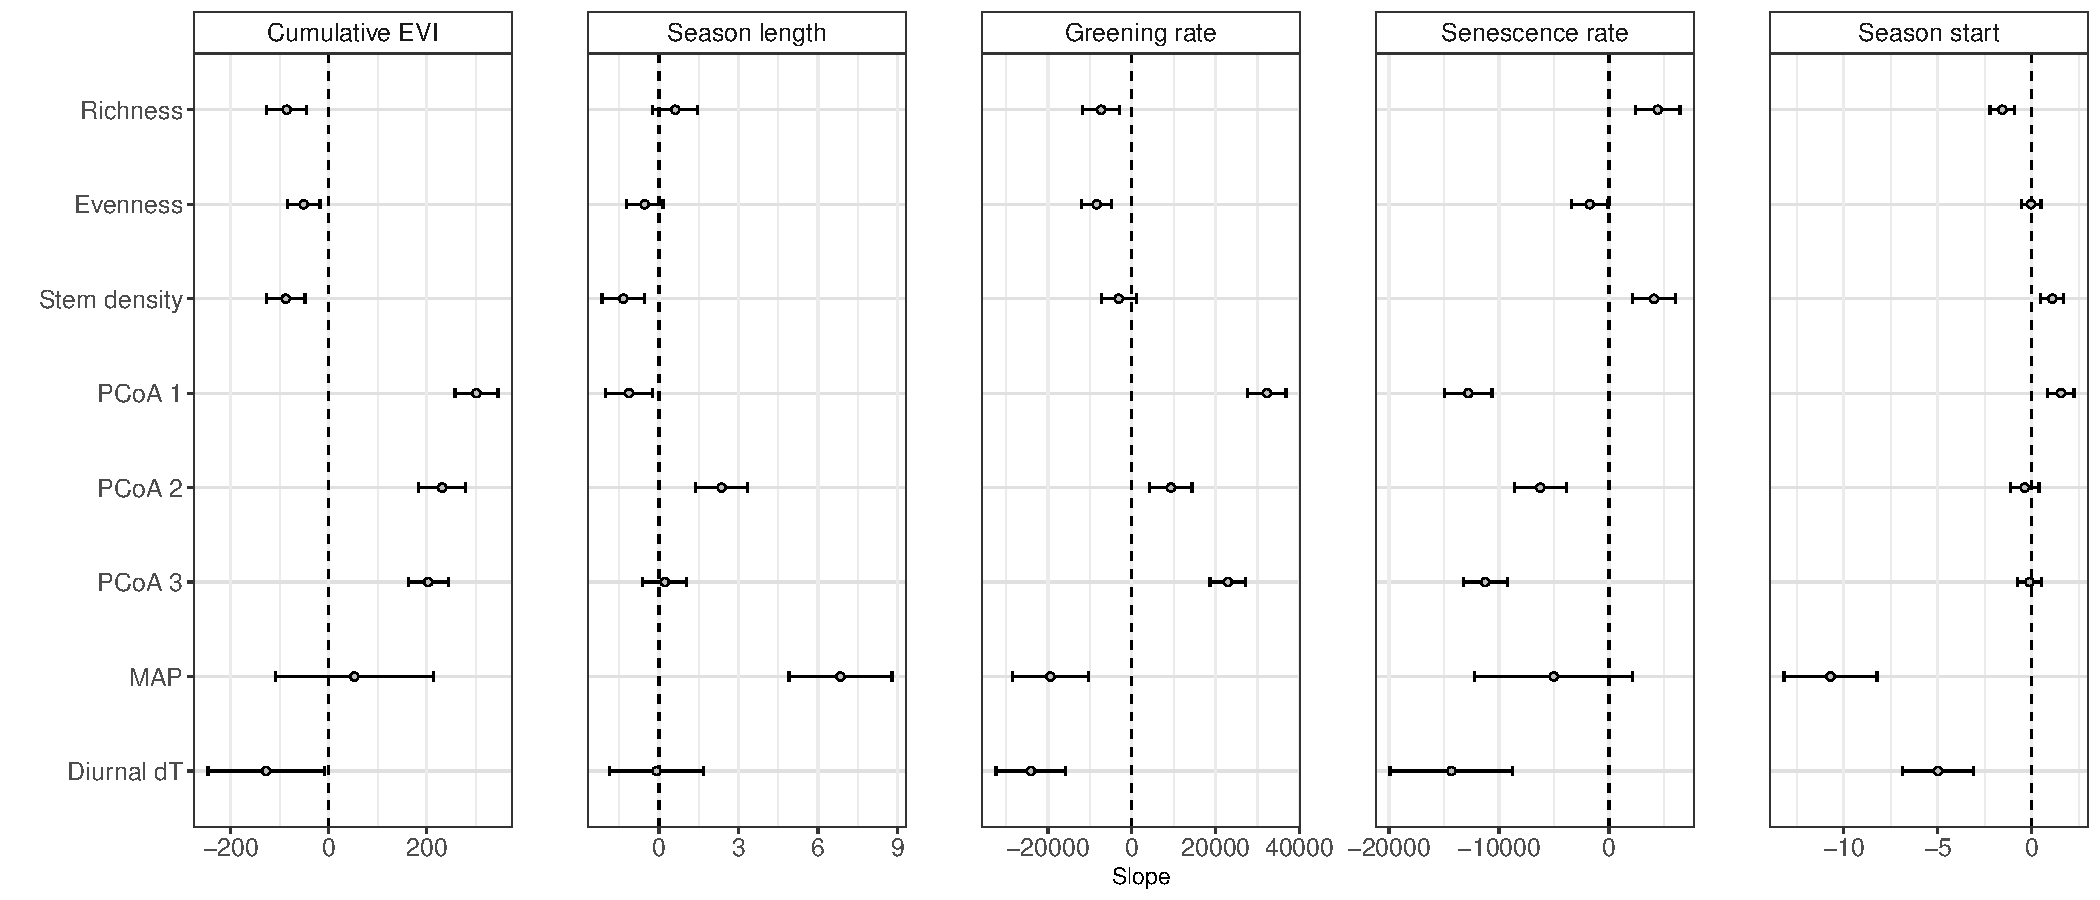
\includegraphics[width=\textwidth]{mod_spamm_slopes.pdf}
	\caption{Predictor slope estimates for each maximal model of a phenological metric. Slope estimates are $\pm$1 standard error. Slope estimates where the interval (standard error) does not overlap zero are considered to be significant effects.}
	\label{mod_spamm_slopes}
\end{figure}

\begin{figure}[H]
\centering
	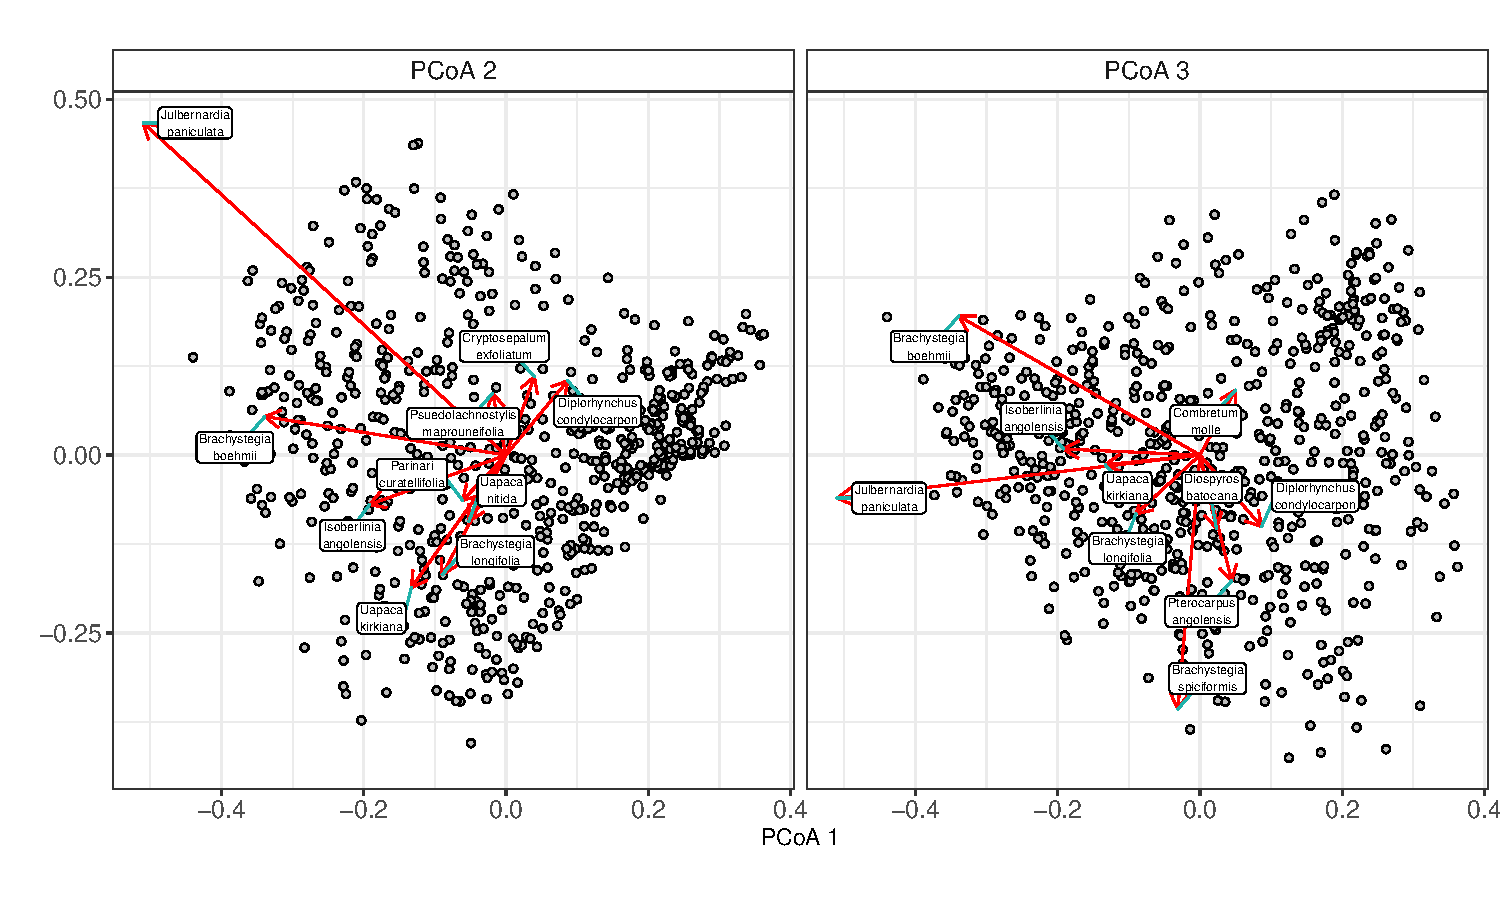
\includegraphics[width=\textwidth]{pcoa.pdf}
	\caption{Species scores fitted to the first and second (A) and first and third (B) axes of the Principal Co-ordinate ordination of tree species composition across all plots. Species vectors are the top ten species by vector length for each axis combination.}
	\label{pcoa}
\end{figure}

\begin{landscape}
\begin{figure}
\centering
	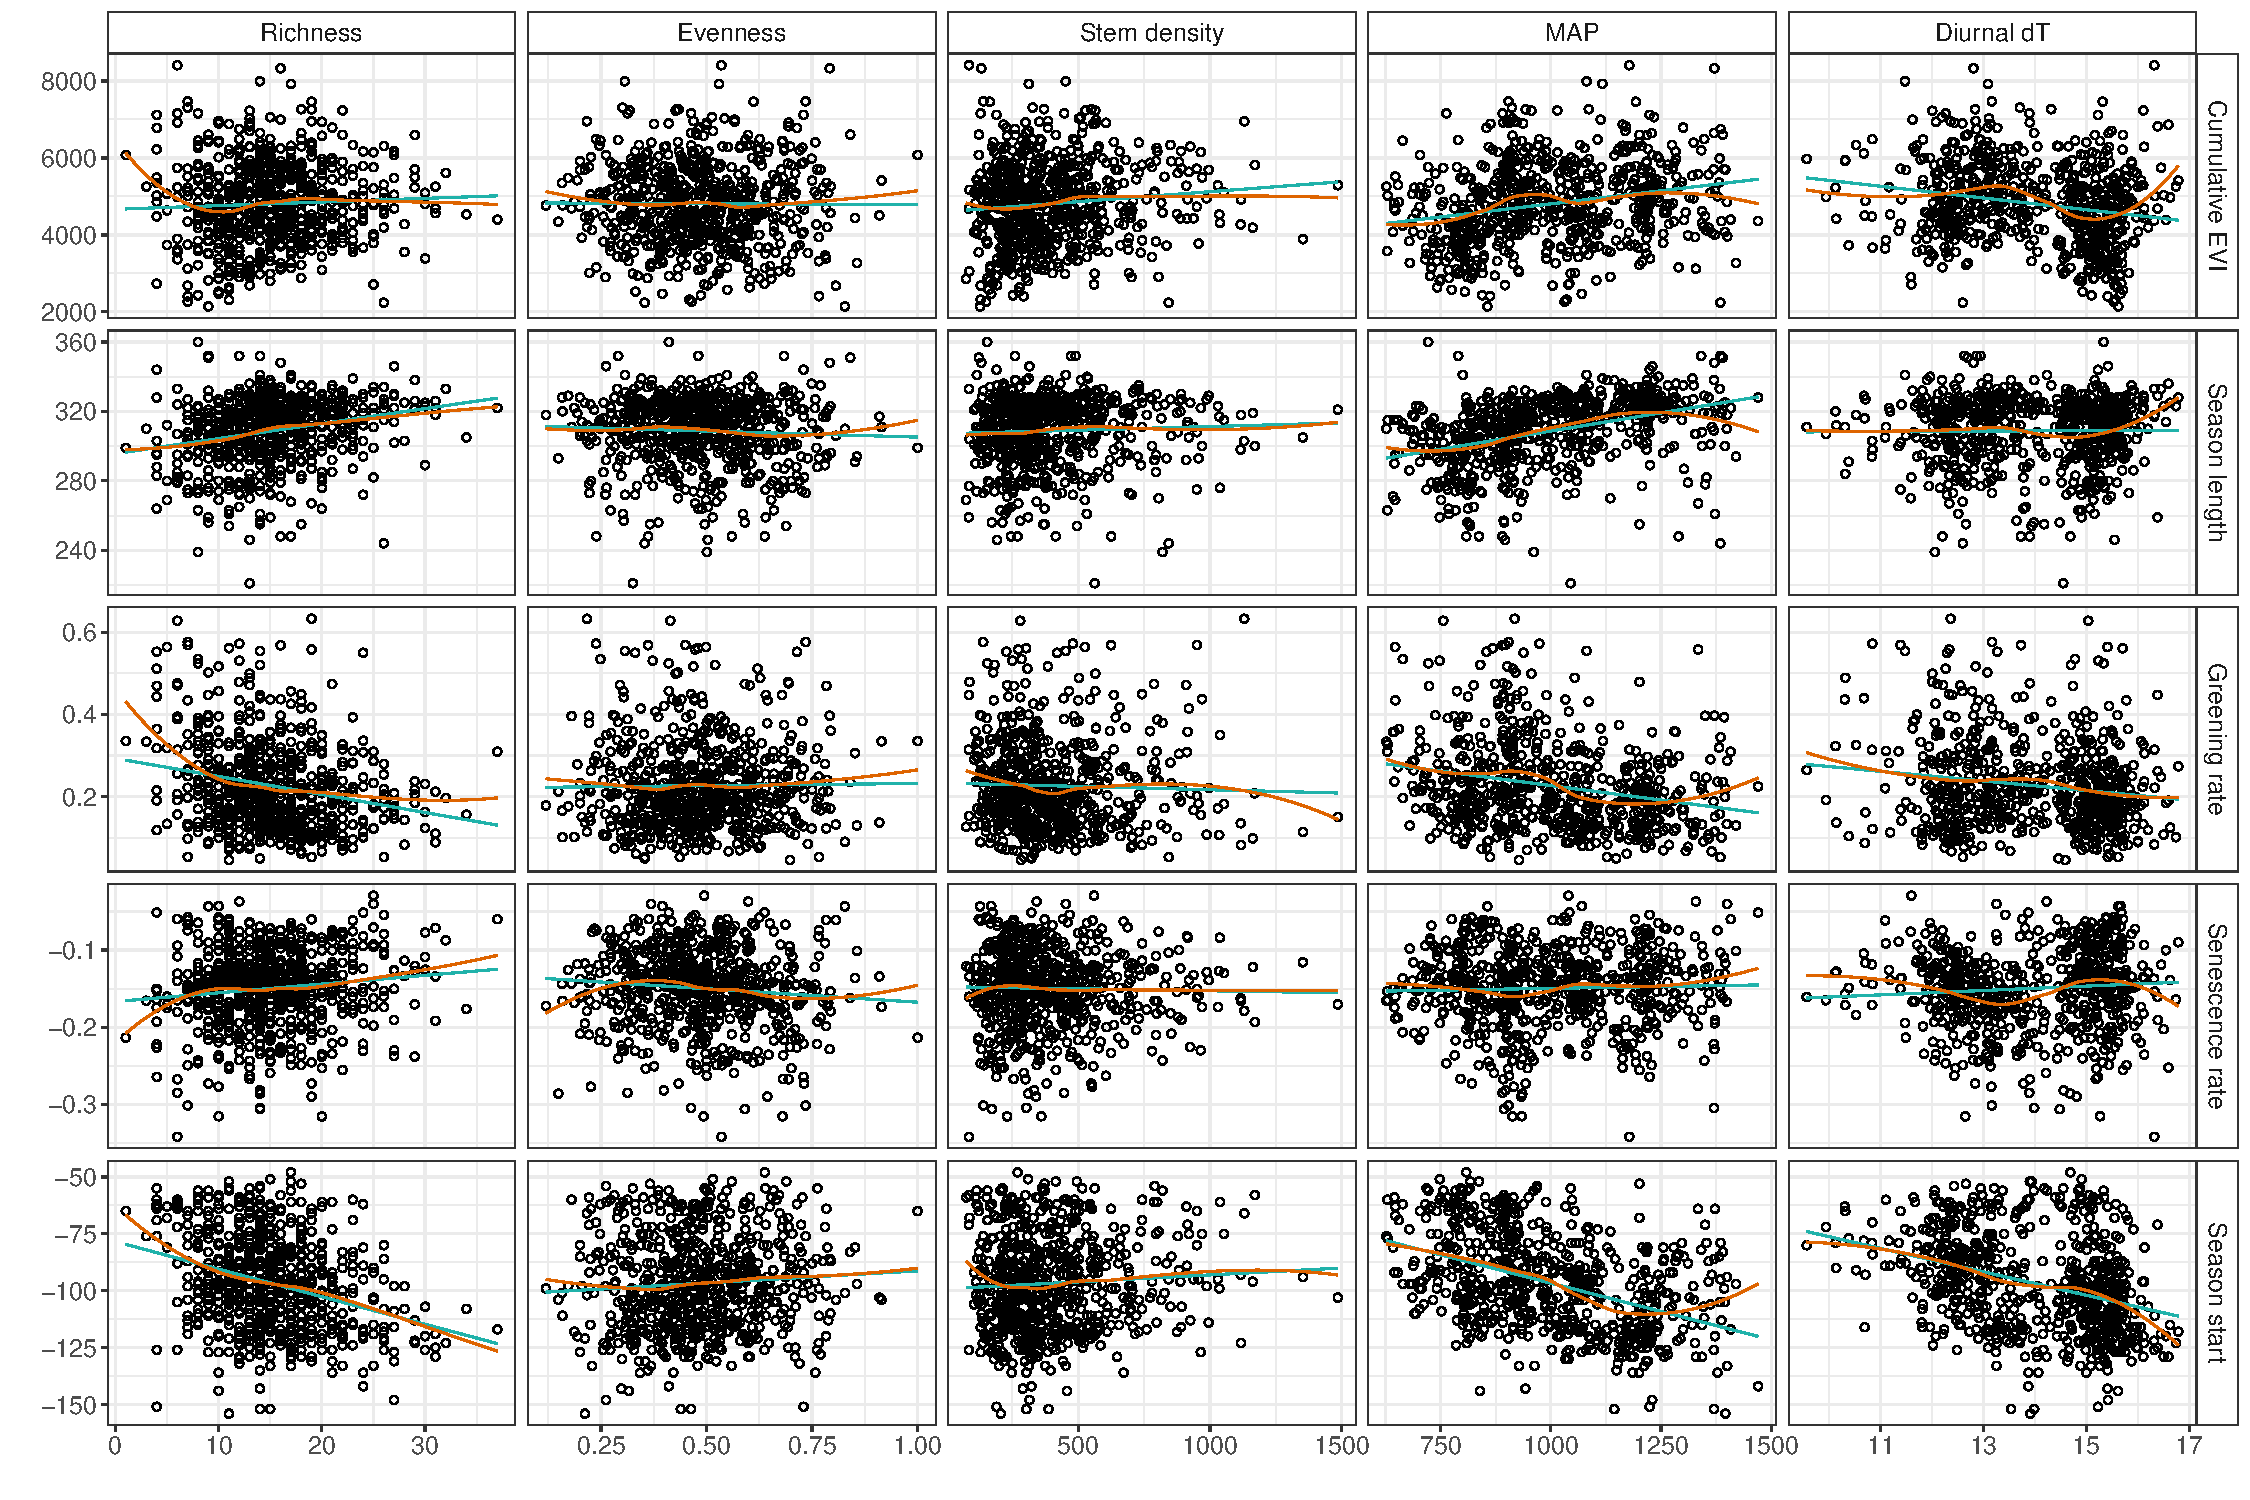
\includegraphics[width=1.4\textwidth]{bivar}
	\caption{Bivariate relationships for model explanatory variables (y) and phenological metrics used as model response variables (x). Blue line of best fit is a linear regression, while the orange line is a loess fit.}
	\label{bivar}
\end{figure}
\end{landscape}

\section{Discussion}

\section{Conclusion}

\bibliography{phenology, include/packages}

\end{document}


